%!TEX root = ../../../super_main.tex
\subsection{Client Requests}
\label{sub:client_requests}
The Android client needs to be able to access these routes somehow and retrieve the information they need to know to send the correct data back to the server as snapshots. There are a few different situations where such a interaction between the client should take place, some will be GUI related and some concerned about retrieving necessary data for the application to do the data gathering. Even though the communication occurs with different purposes most of the aspects of communicating over HTTP, such as establishing a connection and encoding its messages, can be generalized to a common class structure. To simplify the process of these issues we chose to utilize a library, called Webb\footnote{https://github.com/hgoebl/DavidWebb}, handling all the HTTP communication and encoding through a simple interface. Even though we use this library there are still some aspects that can be further generalized, namely ensuring that the communication happens asynchronously and thereby not blocks the applications main thread, ensuring that the right headers and request type is sent, and lastly make some modifications to the TLS verification (see \secref{sec:transport_layer_security}). The way we generalized these aspects were by extending (inheriting from) a class in the Android framework called \mono{AsyncTask} as seen in \figref{fig:async_http_webb_task}, which is an abstract class with an abstract method, named \mono{doInBackground} which is the primary method that is executed in a background thread. Besides the abstract method the class also contains different empty overidable methods that will be called during the tasks life cycle, such as \mono{onPreExecute}, which will be called prior to the execution of the task and \mono{onPostExecute}, which as the name indicates will be called after the execution of the task. Both of these methods will be run on the main thread, which allows them to modify for example GUI elements. 

\begin{figure}[!htbp]
    \centering
    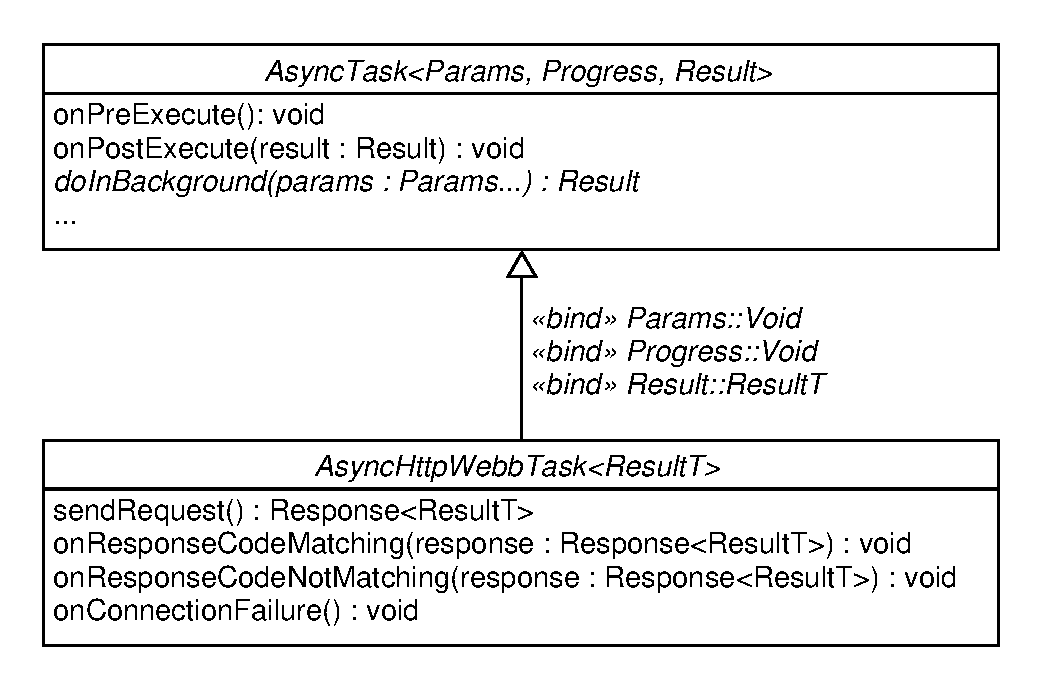
\includegraphics[width=0.5\textwidth]{graphic/architecture/async_http_webb_task.pdf}
    \caption{An UML diagram describing the class extending the AsyncTask.}
    \label{fig:async_http_webb_task}
\end{figure}
\FloatBarrier

We found that we needed to ensure that the response code matches what we expected in the different situations, such as 200 (status OK), and would otherwise need to make some error handling. We also figured that we often would need to specify what to happen if there were no available connection to the server, such that there were no response code returned. Therefore we overrode the \mono{onPostExecute} method as seen in \lstref{lst:on_post_execute}. 

\lstinputlisting[
   style = Java,
   caption = {The \mono{onPostExecute} method, which is called after the asynchronous task has completed.},
   label = {lst:on_post_execute},
   float=!htbp,
]{content/architecture/code_snippets/onPostExecute.java}
\FloatBarrier

Here we firstly check if the response parameter is null, in which case something went wrong in establishing the connection to the server, and the abstract method \mono{onConnectionFailure} will be called. Otherwise we check if the response code matches what we expect, and if it is we call the abstract method \mono{onResponseCodeMatching} and if it does not we call \mono{onResponseCodeNotMatching}. These methods can then be overridden in an anonymous class or a normal class. The response code from the snippet is set through the constructor of the method, along with the the URL the request should be sent to and the request method, which is either ``GET'', ``POST'', ``PUT'', or ``DELETE''. 

\todo[inline]{Skal vi beskrive disse HTTP request typer?}.

The response that the \mono{onPostExecute} in \lstref{lst:on_post_execute} receives as an argument is the result of the doInBackground process, which can be seen in \lstref{lst:do_in_background}. 

\lstinputlisting[
   style = Java,
   caption = {The actual task being executed on a background thread.},
   label = {lst:do_in_background},
   float=!htbp,
]{content/architecture/code_snippets/doInBackground.java}
\FloatBarrier

In this method we firstly create a custom \mono{TrustManager} and \mono{HostnameVerifier}, which is connected to the Transport Layer Security that we utilize and will be described in \secref{sec:transport_layer_security}. This is followed by setting some of the properties that we want to apply to every request, such as adding the ``X-requested-with''-header describing that the request is an Ajax request and not a normal web page request. This is followed by a check of which method is requested in the constructor and use the Webb library to create a request of that type, and use it as a parameter for the abstract method called sendRequest. As with the other abstract methods the \mono{sendRequest} method can be overridden to specify different aspects of the request, such as what the parameters for the request should be as well as how many reties there should be.